\documentclass[10pt,twocolumn,letterpaper]{article}

\usepackage{cvpr}
\usepackage{times}
\usepackage{epsfig}
\usepackage{graphicx}
\usepackage{amsmath}
\usepackage{amssymb}

% Include other packages here, before hyperref.

% If you comment hyperref and then uncomment it, you should delete
% egpaper.aux before re-running latex.  (Or just hit 'q' on the first latex
% run, let it finish, and you should be clear).
\usepackage[breaklinks=true,bookmarks=false]{hyperref}
\usepackage[utf8]{inputenc}

\cvprfinalcopy % *** Uncomment this line for the final submission

\def\cvprPaperID{****} % *** Enter the CVPR Paper ID here
\def\httilde{\mbox{\tt\raisebox{-.5ex}{\symbol{126}}}}

% Pages are numbered in submission mode, and unnumbered in camera-ready
%\ifcvprfinal\pagestyle{empty}\fi
\setcounter{page}{4321}
\begin{document}

%%%%%%%%% TITLE
\title{Computer Vision Lab 05 -Segmentations BSD500}

\author{Juan Carlos Leon Alcazar\\
Universidad de los Andes\\
{\tt\small jc.leon@uniandes.edu.co}
% For a paper whose authors are all at the same institution,
% omit the following lines up until the closing ``}''.
% Additional authors and addresses can be added with ``\and'',
% just like the second author.
% To save space, use either the email address or home page, not both
\and
\\
\\
\\
{\tt\small }
}

\maketitle
%\thispagestyle{empty}


%%%%%%%%% BODY TEXT

\section{Introducción}
El presente laboratorio sirve como introducción al benchmark conocido como 'The Berkeley Segmentation Dataset and Benchmark' (BSD500), un dataset y benchmak público, que abordó por primera vez de forma sistemática y reproducible el problema de segmentación de objetos en imágenes naturales. El objetivo principal de este laboratorio es evaluar un conjunto de métodos de segmentación construidos en el laboratorio previo y compararlos con el método ‘ultrametric contour map’ (UCM) \cite{Arbelaez2009}.

\section{Métodos de segmentación:}
Para  el presente laboratorio se seleccionaron 4 métodos de segmentación:

\begin{description}
\item[KMeans] Construye un conjunto de K clusters según K centroides que minimicen la suma total de las distancias de los puntos a los centroides \footnote{La implementación se encuentra en KmeansSegment.m} \cite{Jain2010}

\item[Mezcla de Gaussianas (GMM)] Construye un conjunto de K clusters donde se tiene un ajuste óptimo de los elementos a un conjunto de K gaussianas (clusters) parametrizadas por un conjunto de K medias y matrices de covarianza. \footnote{Para resolver algunos problemas de convergencia en la implementación de MATLAB se utilizó un regularizador con valor de 0.0001. La implementación se encuentra en GMMSegment.m} \cite{Banfield1993}

\item[Hierachical Cluster] Para cierta distancia D, se crea una jerarquía de elementos que son agrupados  según la similaridad que existe entre ellos. \footnote{Para la implementación de MATLAB se utilizó una distancia euclidiana normalizada por la desviación estándar. La implementación se encuentra en HierachicalSegment.m} \cite{Arifin2006}

\item[Watershed] La imagen es interpretada como una región topográfica, sobre esta región se crean líneas divisorias de agua mediante la inundación simulada de los mínimos locales.  \footnote{Debido a que el método base produce una sobre segmentación  de las imágenes en la base de datos, se agregó una paso de inicialización donde se trata de estimar las regiones de la imagen donde existen objetos grandes y continuos a fin de evitar que el algoritmo de watershed genere clusters en esas regiones. Para este fin  se aplicó un filtro mediano a la imagen (eliminación de bordes espurios) sobre la imagen filtrada se aplicó el detector de bordes de canny y a los bordes se les realizó la operación morfológica de dilatación afin de para expandirlos.  Finalmente el inverso de la imagen fue utilizado como máscara para establecer las regiones donde el. La implementación se encuentra en WatershedSegment.m} \cite{Shafarenko1997}

\end{description}


\subsection{Espacios de segmentación}
Las alternativas para el espacio de color fueron:

\begin{description}
\item[RGB] Es el espacio de color utilizado por múltiples dispositivos electrónicos, los tres canales (rojo, verde y azul) están altamente correlacionados \cite{Forsyth2002}
\item[LAB] Es una extensión del espacio de color CIE XYZ, que además de evitar la correlación entre canales es perceptualmente uniforme.\cite{Forsyth2002}
\item[HSV] Al igual que LAB elimina la correlación entre los tres canales,  contiene información sobre el matiz, saturación y valor del color\cite{Forsyth2002}
\item[Coordenadas] Adicionalmente se utilizaron las coordenadas del pixel para agregar información espacial al proceso de segmentación.  Se tuvo cuidado de  normalizar los valores de color de los pixels (en cualquier espacio) y las coordenadas de tal manera que la magnitud de los dos fuera similar. Esto con el fin de evitar algún sesgo en el proceso de cluster hacia las coordenadas puesto que su rango de valores es mucho más grande que el rango de valores de los espacios de color.
\end{description}
De esta manera se cuenta con 6 espacios de color:

\begin{itemize}
\item RGB
\item LAB
\item HSV
\item RGB+xy
\item LAB+xy
\item HSV+xy
\end{itemize}


\subsection{Selección de los métodos}

Existen 24 combinaciones iniciales de parámetros, se tiene en cuenta los espacios de color y métodos de segmentación (6 espacios de color, 4 métodos de segmentación).

La cantidad de combinaciones aumenta si se considera  el valor de K que a priori puede tomar cualquier valor mayor 2 (1 es un valor válido para cualquier método, pero produciría una segmentación trivial). A fin de estimar un rango de valores adecuado para K, analizamos el número de clusters en el set de ‘train’. Inicialmente calculamos el promedio de clusters de todas las imágenes en set de entrenamiento. Encontramos un promedio de 19.64 clusters, con una desviación estándar de 17.47. Esto indica que el 95\% de las imágenes tiene entre 0 y 55 anotaciones. Con este análisis inicial, una búsqueda exhaustiva de los mejores parámetros posibles implicaría segmentar cada imagen  1320 veces.  En la práctica no se cuenta con tanto tiempo disponible así que utilizamos dos estrategias para reducir el número de pruebas.

Primero, estimamos un rango menor para K, si bien hay imágenes que tienen una gran cantidad de clusters (hasta 95 regiones anotadas) la mayoría de estas regiones cubren un área muy pequeña en la imagen. Con esto en mente, se decidió incluir en el promedio solo aquellos clusters que ocupen más del 2\% de los pixels de la imagen \footnote{No existe una razón formal para elegir el umbral del 2\%, sin embargo, un clúster que agrupa menos del 2\% de los pixels imagen, agruparia menos de 60 pixels; Es poco probable que los métodos utilizados tengan la capacidad de identificar y segmentar una región tan pequeña}

Después de este cambio, se obtiene un promedio de 6.42 clusters por imagen, con una desviación estándar de 3.28. Esto indica que el 95\% de las imágenes tiene entre 2 y  13 clusters . Después de esta reducción se tiene todavía que segmentar cada imagen 244 veces, sumado al tiempo computacional de la evaluación del método, el tiempo de ejecución todavía es prohibitivo.

Para solucionar esto, se aplica una segunda estrategia para evitar hacer pruebas exhaustivas sobre todos los parámetros. Se escoge al azar un subconjunto de 10 imágenes del dataset de ‘test’, aplicar los 4 métodos de segmentación, en 6 espacios de color y para un valor de K que corresponde a  la media (6). A fin de inspeccionar visualmente algunas de las 240 imágenes generadas. El objetivo es tratar de reconocer que combinación de parámetros produce una segmentación que visualmente parece ser más adecuada.

Algunas de las imágenes obtenidas se presentan en las figuras \ref{fig:sRGB}, \ref{fig:SLAB} y \ref{fig:SLABXY}


\begin{figure*}
\begin{center}
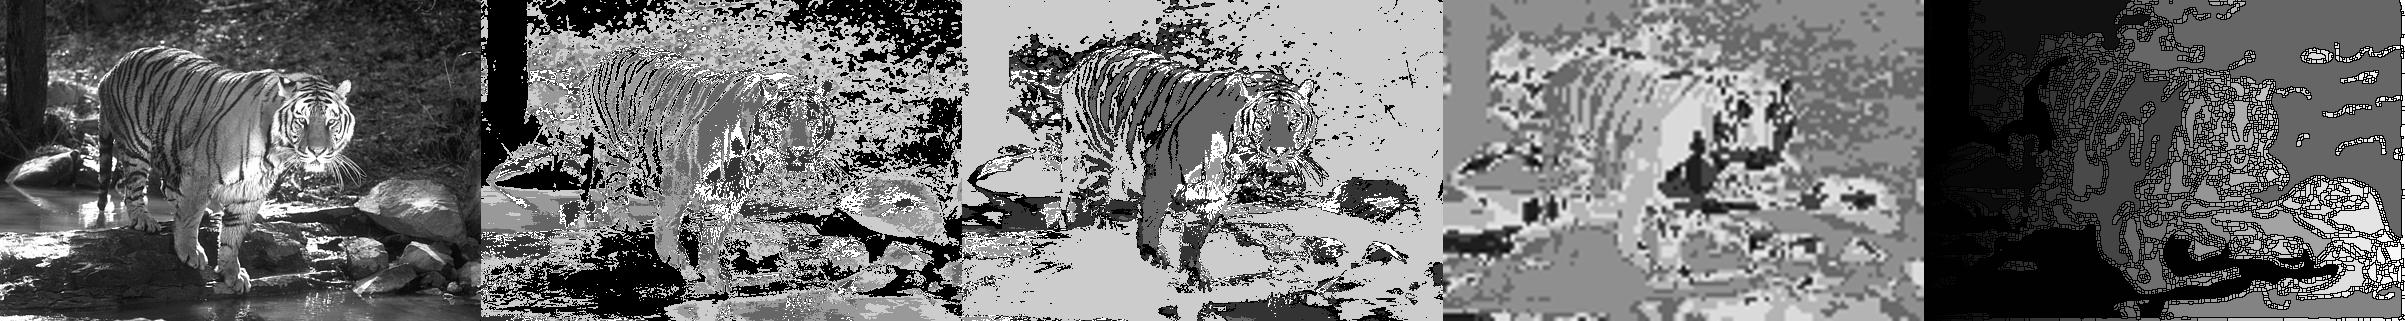
\includegraphics[width=0.95\linewidth]
                {img/RGSample.jpg}
\end{center}
\caption{Segmentación usando RGB de izquierda a derecha: original,Kmeans,GMM,Cluster jerárquico, y watershed. k=6.}
\label{fig:sRGB}
\end{figure*}

\begin{figure*}
\begin{center}
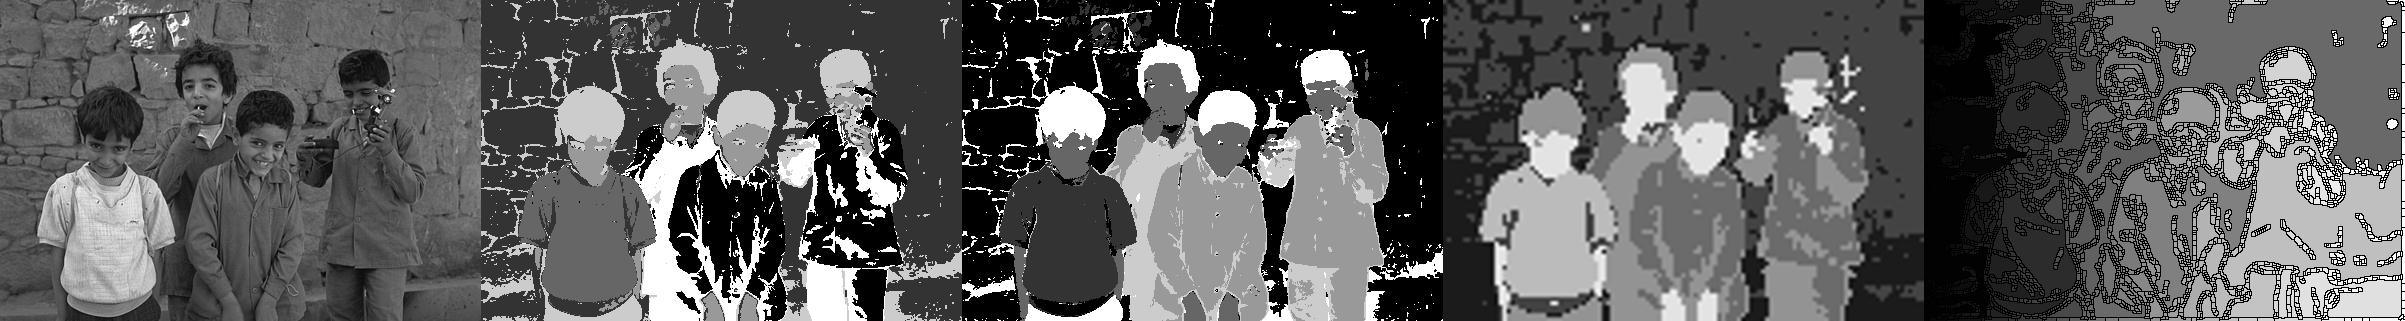
\includegraphics[width=0.95\linewidth]
                {img/LABSample.jpg}
\end{center}
\caption{Segmentación usando LAB de izquierda a derecha: original,Kmeans,GMM,Cluster jerárquico, y watershed. k=6.}
\label{fig:SLAB}
\end{figure*}

\begin{figure*}
\begin{center}
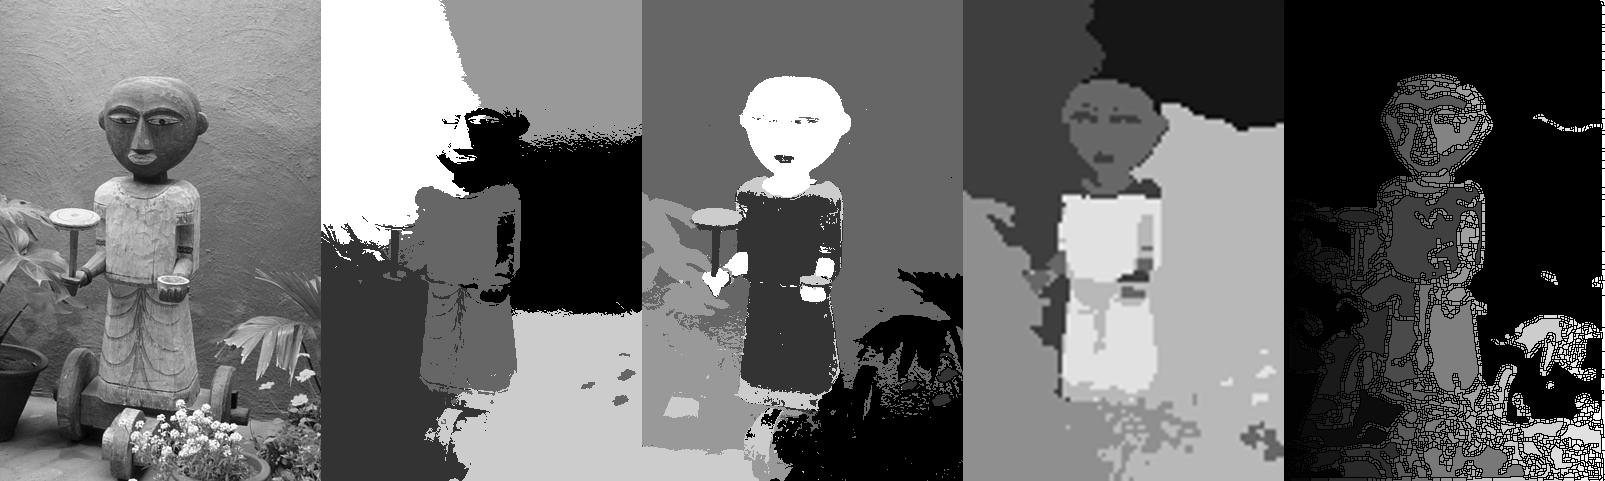
\includegraphics[width=0.95\linewidth]
                {img/LABXYSample.jpg}
\end{center}
\caption{Segmentación usando LAB+xy de izquierda a derecha: original,Kmeans,GMM,Cluster jerárquico, y watershed. k=6.}
\label{fig:SLABXY}
\end{figure*}


Se puede observar que, en general, los resultados de K-Means y Watershed tienden a estar sobre segmentados, (especialmente el caso del watershed). Está sobre segmentación fue el principal argumento para descartar los métodos de K-Means y watershed aun cuando se utilicen los espacios de colores aumentados con las coordenadas xy.

Los resultados del clustering jerárquico y el GMM son muy similares, sin embargo el cluster jerárquico incluye una operación de submuestreo de la imagen (para evitar consumir toda la memoria del computador). Al incrementar el tamaño de la imagen se pierden detalles especialmente el las zonas donde hay bordes o patrones de alta frecuencia espacial. Es posible que esta pérdida de información reduzca el desempeño durante la de evaluación. De esta manera se selecciona como mejor método el GMM.

En cuanto a los espacios de color, la segmentación en el espacio de color RGB es bastante más ruidosa que los espacios de LAB y HSV (ver figura \ref{fig:sRGB} y figura \ref{fig:tiger}), esto se debe, posiblemente, a que los canales de RGB están bastante correlacionados y es poca la información adicional que se puede extraer si se utilizan 2 o 3 canales.

De esta manera se prefieren los espacios de color LAB y HSV sobre RGB. Finalmente la diferencia entre el uso o el no uso de las coordenadas no es evidente en ninguna de las imágenes de prueba, sin embargo, se prefiere el uso de las coordenadas a fin proveer información espacial al método de clustering.


De esta manera la inspección visual concluye con la selección de 2 métodos de clustering
\begin{enumerate}
	\item Espacio de color LAB+xy y cluster por GMM
	\item Espacio de color HSV+xy y cluster por GMM
\end{enumerate}



\section{Dataset y Metodología de pruebas}

La base de datos berkeley BSD500 contiene 500 imágenes  separadas en tres  grupos: training: (200) test (200) y validación (100) todas la imágenes tienen el mismo tamaño 481x321 píxeles, tienen formato jpg, son imágenes a color y se encuentran numeradas para poder ser identificadas dentro del dataset.
La subdivisión del dataset tiene el siguiente objetivo: Sobre el conjunto de ‘train’ se prueba inicialmente los métodos de segmentación y se busca un conjunto de  hiperparametros que permita obtener la mejor segmentación posible. El conjunto de test existe para validar el modelo de aprendizaje y los paramentos encontrados en set de ‘train’ de tal manera que se tengan resultados aceptables dentro de un conjunto de imágenes no visto antes. Cuando se encuentra un modelo e hiperparametros que presentan un buen desempeño tanto en el conjunto de train como el de test, se usa el conjunto de validación para establecer la calidad del método (precisión, exhaustividad y F-Medida en este caso).

\subsection{Verdad de terreno BSD500}

Cada uno de las subdivisiones del dataset cuenta con una ‘verdad de terreno’ (Ground Truth) que se encuentra dentro del directorio ‘..../BSDS500/data/groundTruth’ esta almacenada dentro de archivos binarios con el formato de MATLAB. y está indexada según el número de imagen en la base de datos.  La verdad de terreno de una imagen cualquiera se puede cargar con el comando:\\

‘gt=load('.../BSR/BSDS500/data/groundTruth/2018.mat')’\\

La anotación tiene el mismo tamaño de la imagen original y consta de un único número entero para designar el cluster (el objeto) al que pertenece el píxel. Con ayuda de la función ‘imagesc’ de MATLAB se puede visualizar algunas de las verdades de terreno (ver figura \ref{fig:short2}.

\begin{figure}

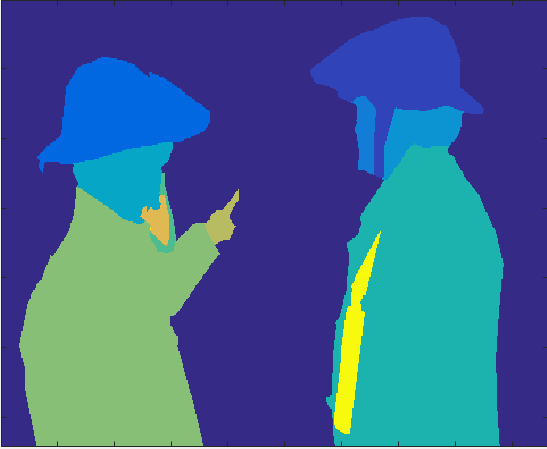
\includegraphics[width=0.85\linewidth]
                {img/Imagesc.png}
\caption{Visualización del ground Truth de una de las imágenes en el dataset}
\label{fig:short2}
\end{figure}

\subsection{Benchmark  BSD500}
El objetivo principal del benchmark construido sobre BSD500 es ofrecer una metodología estandarizada para la evaluación de métodos de segmentación en imágenes naturales. La metodología está basada en la evaluación de las métricas de:
\begin{description}


\item[Precisión] (precisión) esta métrica evalúa la fidelidad de los verdaderos positivos, mientras más cercana sea 1, indica que existe un número bajo de falsos positivos. En este caso nos referimos a elementos clasificados dentro de una región cuando en realidad no pertenece a ella)

\item[Exhaustividad] (recall) esta métrica evalúa qué proporción  de los positivos ha sido marcada como tal. En este caso nos referimos a cuántos elementos que pertenecen a una región no fueron marcados dentro de ella.

\item[F-Medida] (F-MEasure)  es una métrica global que integra la precisión y la exhaustividad. Entregando un puntaje entre 0 y 1. 1 es un puntaje perfecto.
Finalmente el benchmark de BSD500 requiere que se utilicen varias configuración de hiperparametros para así mismo construir varias resultados en la segmentación,  esto con el fin de crear una curva que representa el desempeño del método.
\end{description}

\begin{figure*}
\begin{center}
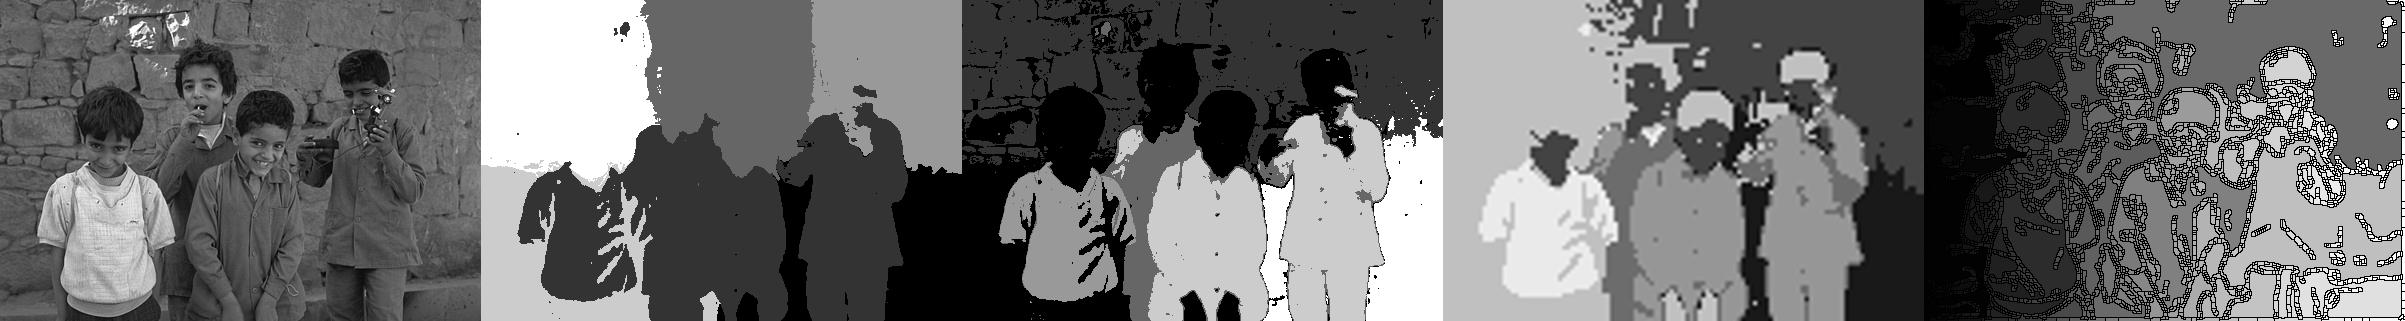
\includegraphics[width=0.95\linewidth]
                {img/Kidshsvxy.jpg}
\end{center}
\caption{Segmentación usando HSV+xy de izquierda a derecha: original,Kmeans,GMM,Cluster jerárquico, y watershed. k=6. Se observa que el método no es capaz de considerar el rosto de las personas y su ropa como un único objeto}
\label{fig:kids}
\end{figure*}

\begin{figure*}
\begin{center}
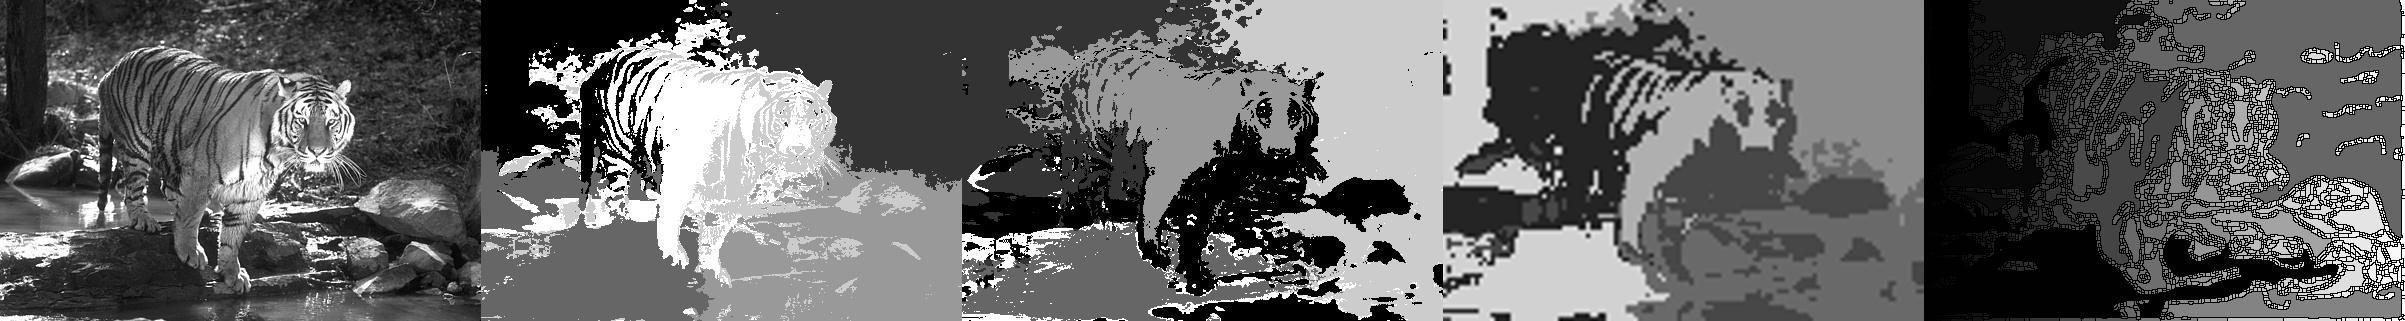
\includegraphics[width=0.95\linewidth]
                {img/Tigerhsvxy.jpg}
\end{center}
\caption{Segmentación usando HSV+xy de izquierda a derecha: original,Kmeans,GMM,Cluster jerárquico, y watershed. k=6. Se observa que el método clasifica las rayas del tigre y su sombra como objetos aparte}
\label{fig:tiger}
\end{figure*}

\begin{figure*}
\begin{center}
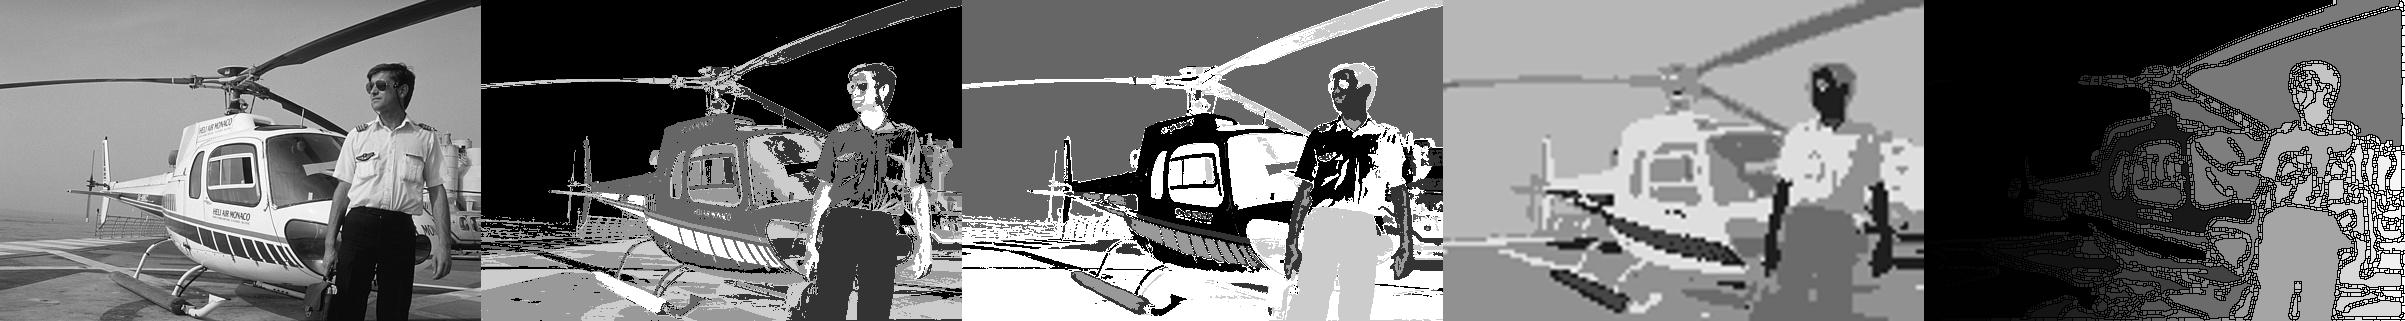
\includegraphics[width=0.95\linewidth]
                {img/Heli.jpg}
\end{center}
\caption{Segmentación usando HSV+xy de izquierda a derecha: original,Kmeans,GMM,Cluster jerárquico, y watershed. k=6. Cambios abruptos de iluminación (como en el vidrio del helicóptero) genera objetos inexistentes}
\label{fig:heli}
\end{figure*}

\begin{figure*}
\begin{center}
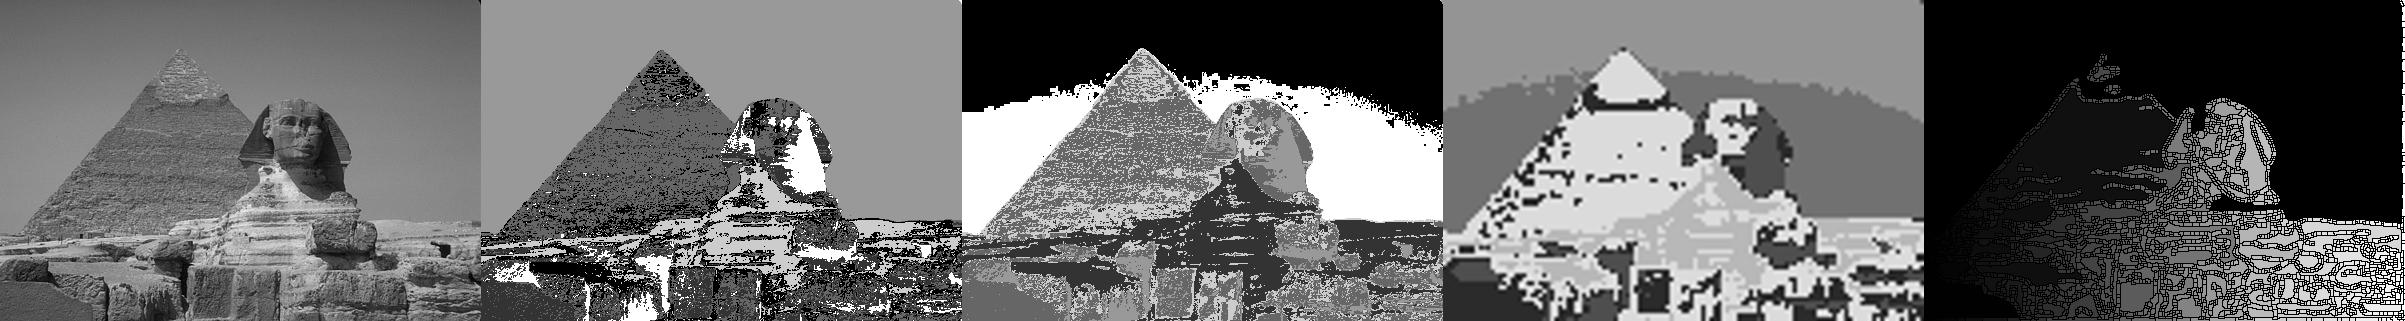
\includegraphics[width=0.95\linewidth]
                {img/Pyramid.jpg}
\end{center}
\caption{Segmentación usando HSV+xy de izquierda a derecha: original,Kmeans,GMM,Cluster jerárquico, y watershed. k=6. Objetos muy grandes como el cielo tienden a ser divididos en varios elementos}
\label{fig:pyra}
\end{figure*}

\begin{figure*}
\begin{center}
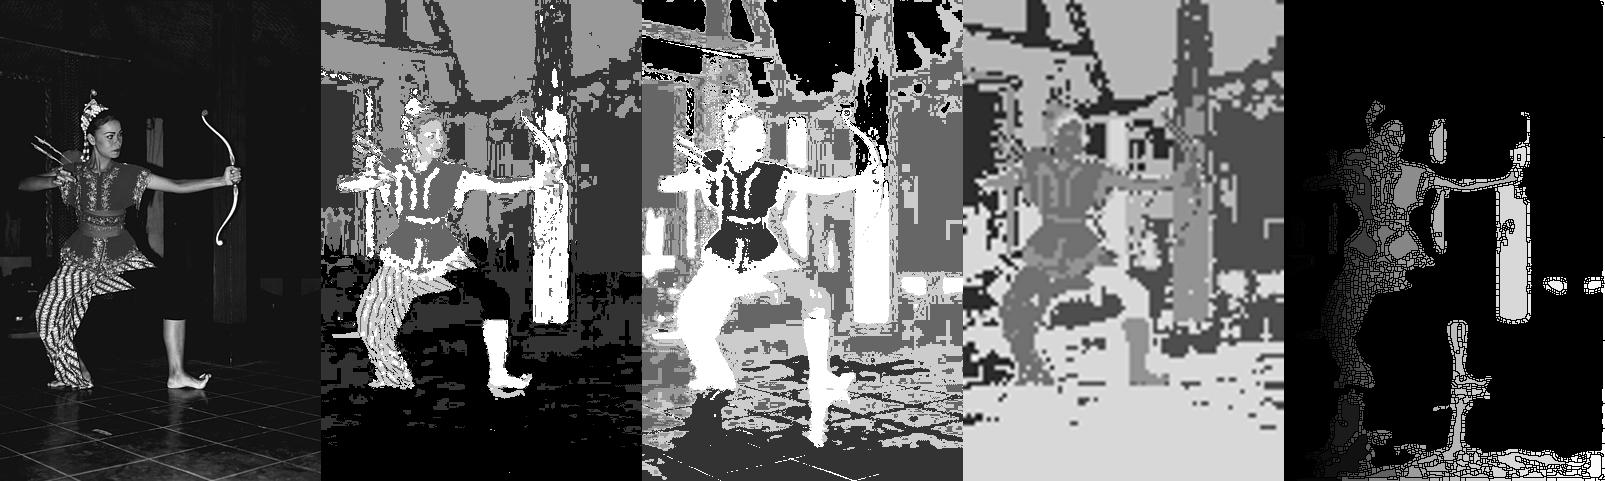
\includegraphics[width=0.95\linewidth]
                {img/woman.jpg}
\end{center}
\caption{Segmentación usando HSV+xy de izquierda a derecha: original,Kmeans,GMM,Cluster jerárquico, y watershed. k=6. Objetos grandes con texturas complejas tienden a ser sobre segmentados}
\label{fig:woman}
\end{figure*}


\section{Resultados}

El benchmark de BSD500 contiene algunos resultados generados con el método ‘ultrametric contour map’ (UCM), para demostrar el uso de la base de datos. Una vez se arreglan los paths para que coincida con la localización de los directorios en el disco local se puede correr sin problema el benchmark 3 que lleva el nombre ‘ 3. boundary benchmark for results stored as a cell of segmentations’.

Los resultados del benchmark con los métodos seleccionados en el laboratorio y el método de UCM sobre el set completo de validación se presentan en la tabla \ref{table:thetable} y la firgura \ref{fig:plot} .


\begin{figure}
\begin{center}
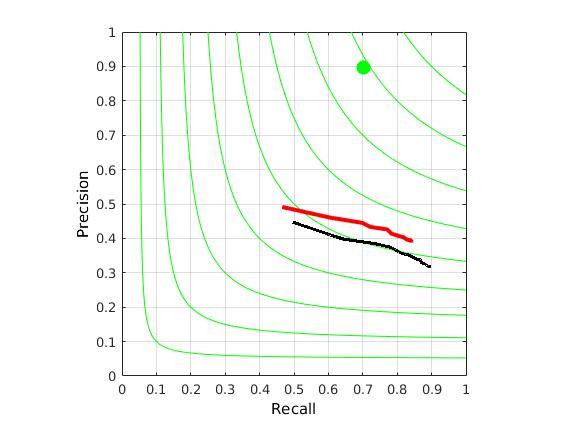
\includegraphics[width=1.15\linewidth]
                {img/metods.jpg}
\end{center}
\caption{Curvas de precision y recall para los métodos usados en el laboratorio. EN negro se tiene la curva de HSV+xy GMM, en rojo la curva de LAB+xy GMM y en magenta la curva del UCM}
\label{fig:plot}
\end{figure}

\begin{table*}[t]
\centering
\begin{tabular}{c | c | c | c }
Metodo & ODS & OID & AreaPR  \\
\hline	
LAB+xy GMM & F( 0.78, 0.38 ) = 0.51  & F( 0.80, 0.45 ) = 0.58 & 0.27 \\
HSV+xy GMM &  &  &  \\
UCM & F( 0.72, 0.70 ) = 0.71  & F( 0.77, 0.71 ) = 0.74 &  0.73\\
\end{tabular}
\label{table:thetable}
\end{table*}


Las curvas obtenidas para los métodos propuestos en este laboratorio comparten la misma deficiencia:  no pueden obtener en ningún caso la precisión de 1.0 (en general nunca es mejor de 0.5) ni la exhaustividad de 1.0 (se acerca a la frontera de 0.9). Esto indica que en ninguna de las combinaciones probadas dentro de este laboratorio (espacio de color y K) se logró un número cercano a cero de falsos positivos o falsos negativos. El desempeño de los dos métodos propuesto es bastante similar, sin embargo, se puede afirmar que la precision del metodo HSV+xy GMM es siempre superior a la del método LAB+xy GMM, a costa de un menor valor de precisión, es decir la segmentación de HSV+xy GMM contiene menos falsos positivos pero a su vez contiene más falsos negativos.


\subsection{Análisis de resultados}

Existe una clara diferencia en desempeño entre los algoritmos creados para el laboratorio y el UCM. La diferencia se puede explicar en gran medida en que los algoritmos utilizan únicamente la información local de color del píxel y la localización absoluta en la imagen. Este tipo de información permite únicamente aproximarse a los verdaderos contornos y tiene varias condiciones de falla entre otras:

\begin{itemize}
\item Si dos regiones del mismo objeto tienen  colores distintos casi siempre son etiquetadas como dos objetos distintos. (ejemplo el rostro y la ropa de una persona, ver figura \ref{fig:kids})
\item  Objetos cuyas texturas tienen patrones con baja frecuencia espacial, tienden a ser divididos según en los patrones que lo conforman (ejemplo las rayas del tigre, ver figura \ref{fig:tiger})
\item Cambios fuertes de iluminación en un objeto de un solo color son clasificados como objetos distintos  (ejemplo el vidrio del helicóptero, ver figura \ref{fig:heli})
\item Tiende a sobre segmentar objetos de gran tamaño cuya textura tiene una alta frecuencia espacial (ver imagen de la mujer con arco \ref{fig:woman})
\item Tiende a dividir los objetos grandes de color aproximadamente constante, (por ejemplo el cielo, ver figura \ref{fig:pyra})

\end{itemize}
Todas estas son fallas muy bien conocidas en los algoritmos de segmentación y, en particular, son fallas que se tuvieron en cuenta al momento de diseñar el algoritmo de UCM.
En la medida que la mayoría de las condiciones de falla están relacionadas con la asignación de un elemento en el cluster equivocado. La precisión del UCM está bastante por encima de lo obtenido por los algoritmos seleccionados.

\subsection{Posibles mejoras sobre el método seleccionado}
En general es muy difícil mejorar el método propuesto sin incluir información extra sobre las regiones que se espera segmentar. En particular información de la continuidad de las regiones (magnitud de gradiente o estimación de bordes) podría ser incorporada dentro del esquema de clustering a fin de evitar la división y unión incorrecta de regiones.

Una segunda falencia del método es que utiliza únicamente la información de local del pixel, en el escenario controlado de BSB esto implica que la información regional del pixel (textura, bordes, esquinas, etc.) es ignorada completamente. En un caso no controlado implica que el ruido de captura y posibles oclusiones van a afectar de manera más severa los resultados.

Finalmente, y para poder superar el desempeño de UCM, sería necesario incorporar información semántica dentro del método, esto permitiría, por ejemplo, que  el rostro y la ropa de una persona se agrupen dentro de un mismo objeto a pesar de no compartir ninguna característica visual. Esto implica que el clustering es solo uno de los pasos dentro de un esquema de clasificación donde se modelan explícitamente las categorías semánticas presentes en la imagen.


\subsection{Aplicación en la práctica}
En un escenario real en el que se requiera aplicar un método de segmentación, no hay razón para preferir alguno de los métodos propuestos por encima del UCM. Existe una muy importante diferencia en el desempeño (especialmente en cuanto a precisión) de los métodos propuestos y UCM. El único caso en el que podría resultar útil el método propuesto es si se requiere una aproximación rápida los posibles objetos de la escena, por ejemplo en la inicialización de un algoritmo de sustracción de fondo.


{\small
\bibliographystyle{ieee}
\bibliography{egbib}
}

\end{document}
